%%%%%%%%%%%%%%%%%%%%%%%%%%%%%%%%%%%%%%%%%%%%%%%%%%%%%%%%%%%%%%%%%%%%%
% Template de Artigo
% XXIX ENMC – Encontro Nacional de Modelagem Computacional
% XVII ECTM – Encontro de Ciência e Tecnologia de Materiais
%%%%%%%%%%%%%%%%%%%%%%%%%%%%%%%%%%%%%%%%%%%%%%%%%%%%%%%%%%%%%%%%%%%%%

\documentclass[12pt,fleqn]{article}

%%%%%%%%%%%%%%%%%%%%%%%%%%%%%%%%%%%%%%%%%%%%%%%%%%%%%%%%%%%%%%%%%%%%%
% CONFIGURAÇÃO DE IDIOMA E CODIFICAÇÃO
%%%%%%%%%%%%%%%%%%%%%%%%%%%%%%%%%%%%%%%%%%%%%%%%%%%%%%%%%%%%%%%%%%%%%

\usepackage[utf8]{inputenc}   % Codificação UTF-8
\usepackage[T1]{fontenc}      % Codificação de fontes
\usepackage[brazil]{babel}    % Português do Brasil (Babel moderno)

%%%%%%%%%%%%%%%%%%%%%%%%%%%%%%%%%%%%%%%%%%%%%%%%%%%%%%%%%%%%%%%%%%%%%
% PACOTES DO TEMPLATE
%%%%%%%%%%%%%%%%%%%%%%%%%%%%%%%%%%%%%%%%%%%%%%%%%%%%%%%%%%%%%%%%%%%%%

\usepackage{setup/config}     % Arquivo de estilo do evento
\usepackage{natbib}           % Sistema de citações
\usepackage{graphicx}         % Inserção de figuras
\usepackage{color}            % Controle de cores
\usepackage{wallpaper}        % Imagens de fundo
\usepackage{hyperref}         % Links e referências
\usepackage{titlesec}         % Controle de títulos
\usepackage{float}            % Permite usar [H] em figuras/tabelas
\usepackage{fancyhdr}         % Cabeçalhos e rodapés

% Seus arquivos
\usepackage[normalem]{ulem}
\usepackage{color}
\usepackage[T1]{fontenc}

% Uso: \comando{texto}, onde 'comando' pode ser 'entra', 'sai', 'rever', 'todo' 
%      ou 
%      \comando[nota adicional]{texto} 

\newcommand{\entra}[2][]{%
   {\color{blue}#2}%
   \ifx&#1&%
      {}% #1 is empty
    \else%
      \footnote{{\color{blue}(entra):} #1}% #1 is nonempty
    \fi%
}%

\newcommand{\sai}[2][]{%
   {\color{black}\sout{#2}}%
   \ifx&#1&%
      {}% #1 is empty
    \else%
      \footnote{{\color{black}(sai):} #1}% #1 is nonempty
    \fi%
}%

\newcommand{\rever}[2][]{%
   {\color{magenta}#2}%
   \ifx&#1&%
      {}% #1 is empty
    \else%
      \footnote{{\color{magenta}(rever):} #1}% #1 is nonempty
    \fi%
}%

\newcommand{\todo}[2][]{%
   {\color{red}[ \textbf{TODO}: \textit{#2} ]}%
   \ifx&#1&%
      {}% #1 is empty
    \else%
      \footnote{{\color{green}(todo):} #1}% #1 is nonempty
    \fi%
}%

\newcommand{\revisor}[2][]{%
   {\color{red}{\bf #2}}%
   \ifx&#1&%
      {}% #1 is empty
    \else%
      \footnote{{\color{red}(revisor):} #1}% #1 is nonempty
    \fi%
}%

\newcommand{\etal}{{\sl et~al.}}

\newcommand{\<}{\textrm{<}}
\renewcommand{\>}{\textrm{>}}


%%%%%%%%%%%%%%%%%%%%%%%%%%%%%%%%%%%%%%%%%%%%%%%%%%%%%%%%%%%%%%%%%%%%%
% DIRETÓRIO DAS FIGURAS
%%%%%%%%%%%%%%%%%%%%%%%%%%%%%%%%%%%%%%%%%%%%%%%%%%%%%%%%%%%%%%%%%%%%%

\graphicspath{{figures/}}

%%%%%%%%%%%%%%%%%%%%%%%%%%%%%%%%%%%%%%%%%%%%%%%%%%%%%%%%%%%%%%%%%%%%%
% AJUSTE DE ESPAÇAMENTO NA BIBLIOGRAFIA
%%%%%%%%%%%%%%%%%%%%%%%%%%%%%%%%%%%%%%%%%%%%%%%%%%%%%%%%%%%%%%%%%%%%%

% Reduz espaçamento entre referências
\let\OLDthebibliography\thebibliography
\renewcommand\thebibliography[1]{%
\OLDthebibliography{#1}
\setlength{\parskip}{0pt}
\setlength{\itemsep}{0pt plus 0.3ex}
}

%%%%%%%%%%%%%%%%%%%%%%%%%%%%%%%%%%%%%%%%%%%%%%%%%%%%%%%%%%%%%%%%%%%%%
% TÍTULO DO ARTIGO
%%%%%%%%%%%%%%%%%%%%%%%%%%%%%%%%%%%%%%%%%%%%%%%%%%%%%%%%%%%%%%%%%%%%%

\title{INTELIGÊNCIA ARTIFICIAL APLICADA À DETECÇÃO DE CAPRINOS EM AMBIENTE CONFINADO}

%%%%%%%%%%%%%%%%%%%%%%%%%%%%%%%%%%%%%%%%%%%%%%%%%%%%%%%%%%%%%%%%%%%%%
% AUTORES E AFILIAÇÕES
%%%%%%%%%%%%%%%%%%%%%%%%%%%%%%%%%%%%%%%%%%%%%%%%%%%%%%%%%%%%%%%%%%%%%

\author{
\rm
\begin{tabular}{l}
\textbf{Vinícius Latini Gonçalves}$^{1}$ - {\textnormal vinicius.latini@estudante.ufjf.br}\\
\textbf{Gabriel Vaz Bernardini Ferreira}$^{2}$ - {\textnormal gabrielbr1809@aluno.ufsj.com.br}\\
\textbf{Felipe Girardi Siqueira}$^{2}$ - {\textnormal felipeprinci@aluno.ufsj.edu.br}\\
\textbf{Luciana Conceição D. Campos}$^{1}$ - {\textnormal luciana.campos@ufjf.br}\\
\textbf{Érica da Costa Reis Carvalho}$^{2}$ - {\textnormal ericacarvalho@ufsj.edu.br}\\
\textbf{Acir Moreno Soares Júnior}$^{2}$ - {\textnormal acir@ufsj.edu.br}\\
{\fontsize{11}{0}\selectfont $^{1}$Universidade Federal de Juiz de Fora, Juiz de Fora – MG}\\
{\fontsize{11}{0}\selectfont $^{2}$Universidade Federal de São João del-Rei, São João del-Rei – MG}\\
\end{tabular}
}

%%%%%%%%%%%%%%%%%%%%%%%%%%%%%%%%%%%%%%%%%%%%%%%%%%%%%%%%%%%%%%%%%%%%%
% RODAPÉ ESPECIAL DA PRIMEIRA PÁGINA
%%%%%%%%%%%%%%%%%%%%%%%%%%%%%%%%%%%%%%%%%%%%%%%%%%%%%%%%%%%%%%%%%%%%%

\fancypagestyle{firstpagestyle}
{
\renewcommand{\headrulewidth}{0pt}

\fancyfoot[C]{
\footnotesize
\parbox{15cm}{
\centering
\fontsize{7.5}{0}\selectfont\it
XXIX ENMC – Encontro Nacional de Modelagem Computacional\\
XVII ECTM – Encontro de Ciência e Tecnologia de Materiais\\
06 a 09 de outubro de 2026 - Bento Gonçalves - RS
}}
}

%%%%%%%%%%%%%%%%%%%%%%%%%%%%%%%%%%%%%%%%%%%%%%%%%%%%%%%%%%%%%%%%%%%%%
% INÍCIO DO DOCUMENTO
%%%%%%%%%%%%%%%%%%%%%%%%%%%%%%%%%%%%%%%%%%%%%%%%%%%%%%%%%%%%%%%%%%%%%

\begin{document}

\pretolerance=10000

%%%%%%%%%%%%%%%%%%%%%%%%%%%%%%%%%%%%%%%%%%%%%%%%%%%%%%%%%%%%%%%%%%%%%
% LOGO DO EVENTO
%%%%%%%%%%%%%%%%%%%%%%%%%%%%%%%%%%%%%%%%%%%%%%%%%%%%%%%%%%%%%%%%%%%%%

\begin{figure}
\centering

\includegraphics[width=6.25in]{logo.png}
\end{figure}

\vspace{-3cm}

%%%%%%%%%%%%%%%%%%%%%%%%%%%%%%%%%%%%%%%%%%%%%%%%%%%%%%%%%%%%%%%%%%%%%
% TÍTULO
%%%%%%%%%%%%%%%%%%%%%%%%%%%%%%%%%%%%%%%%%%%%%%%%%%%%%%%%%%%%%%%%%%%%%

\maketitle

\pagestyle{empty}
\thispagestyle{firstpagestyle}

%%%%%%%%%%%%%%%%%%%%%%%%%%%%%%%%%%%%%%%%%%%%%%%%%%%%%%%%%%%%%%%%%%%%%
% RESUMO
%%%%%%%%%%%%%%%%%%%%%%%%%%%%%%%%%%%%%%%%%%%%%%%%%%%%%%%%%%%%%%%%%%%%%
\begin{abstract}
O uso de sistemas baseados em Visão Computacional tem se expandido consideravelmente nos últimos anos, com aplicações promissoras na chamada zootecnia de precisão, incluindo o monitoramento e a análise automatizada de animais em ambientes de confinamento. Apesar da ampla disponibilidade de recursos tecnológicos, ainda existem desafios relacionados à aplicação desses sistemas em condições reais, especialmente diante de variações de perspectiva e iluminação. Nesse contexto, este trabalho propõe uma arquitetura baseada em Mistura de Especialistas (\textit{Mixture of Experts} -- MoE) para a detecção de caprinos da raça \textit{Saanen} em ambiente de confinamento. A abordagem combina uma rede de roteamento (\textit{gating network}) baseada em \textit{EfficientNet} -- responsável exclusivamente pela classificação do cenário de captura (perspectiva e condição de iluminação), e não pela classificação do animal -- com quatro modelos YOLOv8 especializados, cada um dedicado à detecção da classe única \texttt{goat} em uma combinação específica de perspectiva e iluminação. Para o treinamento e a avaliação dos detectores, foram utilizados vídeos capturados em ambientes experimentais da Universidade Federal de São João del-Rei, a partir dos quais foi construído um banco de imagens rotuladas com uma única classe, \texttt{goat}. Os resultados indicaram elevado desempenho dos modelos especialistas nos quatro cenários avaliados, demonstrando a viabilidade da estratégia modular para a detecção de caprinos em condições distintas de captura.
\end{abstract}
%%\begin{abstract} O uso de sistemas baseados em Visão Computacional tem se expandido consideravelmente nos últimos anos, com aplicações promissoras na chamada zootecnia de precisão que vão desde o controle de atividades básicas de inspeção de qualidade até a análise de comportamento para a garantia do bem estar animal (BEA) e sanidade do rebanho. Apesar da ampla disponibilidade de recursos tecnológicos, ainda há desafios relacionados à montagem, configuração, custo e aplicação desses sistemas em ambientes reais. Nesse sentido, o presente trabalho propõe o desenvolvimento de um sistema de baixo custo, baseado em Visão Computacional e Inteligência Artificial, para detecção e classificação de cabras da raça Saanen em confinamento a partir da análise de diferentes modelos de aprendizado de máquina. A iniciativa proposta integra conhecimentos das áreas de Ciência da Computação e Zootecnia, utilizando vídeos capturados em ambientes experimentais para a construção de um banco de imagens rotuladas com vistas ao treinamento e avaliação dos modelos propostos para operação com recursos computacionais limitados. Dessa forma,  espera-se contribuir para a construção de ferramentas especializadas que possam auxiliar tanto na detecção quanto na classificação desses animais. \end{abstract}

\keywords{\em{Inteligência Artificial, Visão Computacional, Detecção de Objetos, Mistura de Especialistas (MoE), Zootecnia de Precisão.}}

%%%%%%%%%%%%%%%%%%%%%%%%%%%%%%%%%%%%%%%%%%%%%%%%%%%%%%%%%%%%%%%%%%%%%
% CABEÇALHO DAS DEMAIS PÁGINAS
%%%%%%%%%%%%%%%%%%%%%%%%%%%%%%%%%%%%%%%%%%%%%%%%%%%%%%%%%%%%%%%%%%%%%

\fancyhead[L]{\footnotesize{\fontsize{7.5}{0}\selectfont\it
XXIX ENMC, XVII ECTM\\
06 a 09 de outubro de 2026}}

\renewcommand{\headrulewidth}{0pt}

\fancyfoot[C]{
\footnotesize
\parbox{15cm}{
\centering
\fontsize{7.5}{0}\selectfont\it
XXIX ENMC – Encontro Nacional de Modelagem Computacional\\
XVII ECTM – Encontro de Ciência e Tecnologia de Materiais\\
06 a 09 de outubro de 2026 - Bento Gonçalves - RS
}}

\rhead{}

\pagestyle{fancy}

%%%%%%%%%%%%%%%%%%%%%%%%%%%%%%%%%%%%%%%%%%%%%%%%%%%%%%%%%%%%%%%%%%%%%
% INÍCIO DO TEXTO
%%%%%%%%%%%%%%%%%%%%%%%%%%%%%%%%%%%%%%%%%%%%%%%%%%%%%%%%%%%%%%%%%%%%%

\section{INTRODUÇÃO}

O uso de sistemas baseados em Visão computacional e Inteligência artificial tem se expandido consideravelmente nos últimos anos, especialmente no contexto da agricultura de precisão e do manejo zootécnico. Essas tecnologias vêm possibilitando o desenvolvimento de soluções inovadoras para o controle de atividades em ambientes rurais e experimentais, com aplicações que vão desde a inspeção de qualidade \citep{industrial_quality_cv_2024}, análise de comportamento animal \cite{animalformer_2024} e monitoramento de cultivos \cite{vit_precision_agriculture_2025}, até a automação de processos \cite{kang2025bokchoy_cv_iot}. Por serem acessíveis, precisas e não invasivas, tais inovações contribuem para a adoção de práticas mais eficientes e sustentáveis.


Entretanto, apesar da ampla disponibilidade de recursos tecnológicos, ainda há desafios relacionados à montagem, configuração e aplicação desses sistemas em ambientes reais. Além disso, a construção de bancos de dados anotados ou rotulados (\textit{datalogs}) e o treinamento de algoritmos de aprendizado de máquina requerem conhecimentos específicos e tempo dedicado.

Na Universidade Federal de São João del-Rei (UFSJ), essa abordagem está sendo explorada no projeto interdisciplinar “Inteligência artificial aplicada à detecção e classificação comportamental de cabras em confinamento (raça \textit{Saanen})”, envolvendo docentes e discentes dos cursos de Zootecnia e Ciência da Computação. O presente artigo situa-se especificamente no módulo de detecção desse projeto guarda-chuva; as etapas de classificação comportamental dos animais não fazem parte do escopo deste trabalho, permanecendo como direção de pesquisas futuras vinculadas ao projeto. Os avanços em Visão Computacional e em técnicas de aprendizado profundo têm ampliado as possibilidades de desenvolvimento de sistemas automatizados para captura, processamento e análise de vídeos e imagens em aplicações de monitoramento animal.

%Os avanços em Visão computacional, aliados à popularização de \textit{hardwares} de baixo custo como o Raspberry Pi\footnote{O Raspberry Pi é um minicomputador de baixo custo amplamente utilizado em projetos educacionais e protótipos de \textit{hardware}.} e o Arduino\footnote{O Arduino é uma plataforma de prototipagem eletrônica baseada em \textit{hardware} e \textit{software} livres, muito usada para controlar sensores e atuadores em projetos embarcados.} \cite{arablouei2021animal_embedded}, tornaram possível o desenvolvimento de sistemas embarcados que capturam, processam e analisam vídeos e imagens em tempo real.

Um dos aspectos fundamentais para o bem-estar animal na pecuária é a garantia de um ambiente adequado, com alimentação e água em quantidade e qualidade suficientes, o que demanda uma quantidade significativa de horas de trabalho humano. Com o avanço da ciência e da tecnologia no século XXI, bem como com o aumento das exigências dos consumidores por produtos de origem animal de alta qualidade, torna-se cada vez mais necessário o aprimoramento dos métodos de monitoramento da produção pecuária \citep{dominiak2019, nasirahmadi2017, halachmi2019}. O desenvolvimento e a integração de novas tecnologias, como sensores em tempo real e sistemas de análise de dados multissensoriais, têm possibilitado a obtenção e interpretação de informações de forma mais eficiente, reduzindo o tempo de processamento e facilitando o acesso a dados relevantes tanto para produtores quanto para pesquisadores. 

Nesse contexto, diversas pesquisas já demonstraram a viabilidade do monitoramento automático do comportamento animal, muitas vezes aliado à análise de características comportamentais e fisiológicas \cite{halachmi2019, fogarty2018}. Tais abordagens tecnológicas têm contribuído significativamente para a identificação de padrões normais e anormais no comportamento dos animais, promovendo melhorias no manejo e no bem-estar dos rebanhos.

Este trabalho tem como objetivo desenvolver e avaliar uma arquitetura baseada em Mistura de Especialistas (\textit{Mixture of Experts} -- MoE) para a detecção automatizada, com classe única (\texttt{goat}), de caprinos da raça \textit{Saanen} em ambientes de confinamento sujeitos a diferentes condições de perspectiva e iluminação. Para isso, propõe-se uma rede de roteamento (\textit{gating network}), baseada em \textit{EfficientNet}, cuja função é exclusivamente classificar o cenário de captura (perspectiva e condição de iluminação) -- sem realizar classificação do animal -- e direcionar cada entrada a um dentre quatro detectores YOLOv8 especializados, cada qual responsável pela detecção da classe única \texttt{goat} em uma combinação específica de perspectiva (frontal ou superior) e iluminação (diurna ou noturna). Como objetivos específicos, busca-se: (i) construir e organizar uma base de imagens rotuladas de caprinos, com classe única \texttt{goat}, para os quatro cenários de captura; (ii) treinar e avaliar detectores YOLOv8 especializados por cenário; e (iii) integrar os especialistas a uma rede de roteamento (\textit{gating network}) que realiza a seleção automática do detector mais adequado durante a inferência, a partir da classificação do cenário de captura.

%%Este trabalho, portanto, tem como objetivo explorar e desenvolver soluções de baixo custo para identificação e classificação de imagens de animais caprinos da raça \textit{Saanen} em confinamento, promovendo sua aplicação prática em ambientes de pesquisa da UFSJ. Busca-se, com isso, a construção de sistemas computacionais eficazes para a detecção de caprinos. Este trabalho está em consonância com a Agenda 2030 da ONU, especialmente com os Objetivos de Desenvolvimento Sustentável ODS 2 (Fome Zero e Agricultura Sustentável), ODS 9 (Inovação e Infraestrutura) e ODS 12 (Consumo e Produção Responsáveis), ao propor um sistema tecnológico eficiente para o monitoramento de caprinos com foco em bem-estar animal e produtividade sustentável \cite{rohan2023deep_livestock_survey, rifqie2025goat_counting_edge}.

\section{METODOLOGIA}

A abordagem metodológica proposta para a automatização da detecção de caprinos da raça \textit{Saanen} em ambientes de confinamento foi estruturada em quatro etapas fundamentais: a constituição e rotulação do \textit{dataset} experimental; a estratégia de validação baseada em \textit{K-Fold Cross-Validation}; a especificação e parametrização dos modelos YOLOv8 especialistas, definindo um procedimento de treinamento consistente e padronizado para cada cenário; e, por fim, a concepção de uma arquitetura baseada em Mistura de Especialistas (\textit{Mixture of Experts} - MoE). A seguir serão apresentados os detalhes de cada etapa.

%%A abordagem metodológica proposta para a automatização da detecção e classificação de caprinos da raça Saanen em ambientes de confinamento foi estruturada em quatro etapas fundamentais: a constituição e rotulação do \textit{dataset} experimental; a estratégia de validação baseada em \textit{K-Fold Cross-Validation}; a especificação e parametrização dos modelos YOLOv8 especialistas, definindo um procedimento de treinamento consistente e padronizado para cada cenário; e, por fim, a concepção de uma arquitetura baseada em Mistura de Especialistas (\textit{Mixture of Experts} - MoE). A seguir serão apresentados os detalhes de cada etapa.

\subsection{Aquisição e Preparação da Base de Dados}
\label{subsec:aquisicao_dados}

Os dados utilizados neste trabalho foram obtidos a partir de registros de vídeo capturados em ambientes experimentais de confinamento, fruto de uma cooperação interdisciplinar envolvendo os cursos de Zootecnia e Ciência da Computação da UFSJ. Os cenários foram monitorados por quatro câmeras fixas (\texttt{Cam01} a \texttt{Cam04}), posicionadas de forma a registrar os espécimes sob diferentes ângulos (perspectivas frontal e superior) e condições de iluminação (diurna, com luz natural, e noturna, sob espectro infravermelho). Os vídeos foram capturados na resolução nativa de 1280$\times$960 pixels, a uma taxa de 8 quadros por segundo (\textit{frames per second} -- FPS), ao longo de 36 sessões de gravação distintas, distribuídas em 7 dias de aquisição e realizadas em diferentes horários durante o período experimental. Todos os quadros de cada sessão foram extraídos e preservados no conjunto de dados, sem subamostragem adicional além da taxa nativa de captura. O rebanho monitorado é composto por 8 indivíduos da raça \textit{Saanen}, mantidos na mesma baia em todos os cenários de captura. Para o treinamento dos detectores, os quadros extraídos foram redimensionados para $640 \times 640$ pixels, resolução de entrada padrão da arquitetura YOLOv8.

O processo de rotulação das imagens foi executado manualmente com o auxílio de uma ferramenta desenvolvida pelos alunos da UFSJ, denominada \textit{EasyLabel}\footnote{https://github.com/Gabriel0Bernardini/EasyLabel?tab=readme-ov-file}. Foi definida uma classe única alvo denominada \texttt{goat}, delimitada por caixas envolventes (\textit{bounding boxes}) ajustadas de forma justa para minimizar espaços vazios. As anotações geraram ficheiros \texttt{.txt} no formato padrão requerido pela arquitetura YOLO, contendo o identificador da classe seguido pelas coordenadas normalizadas do centro da caixa, largura e altura:
\begin{equation}
    \text{class\_id} \quad \; \; \text{center}_x \quad \; \; \text{center}_y \quad \; \; \text{width} \quad \; \; \text{height},
\end{equation}
%
onde todos os valores espaciais encontram-se mapeados no intervalo $[0, 1]$. Vale ressaltar que esse processo foi realizado por alunos da UFSJ que criaram uma API capaz de gerar os \textit{datasets} de forma otimizada utilizando o método e formato mencionado anteriormente.

A Tabela~\ref{tab:dataset_caracterizacao} apresenta a distribuição quantitativa do conjunto de dados de detecção entre os quatro cenários operacionais que fundamentam a arquitetura MoE, consolidando o volume de imagens, o total de caixas delimitadoras anotadas e o número de sessões de vídeo independentes utilizadas em cada especialista.

\begin{table}[H]
\caption{Caracterização do Dataset de Detecção por Cenário Operacional.}
\label{tab:dataset_caracterizacao}
\centering{}
\begin{tabular*}{\textwidth}{@{\extracolsep{\fill}}lccccc}
\hline
Cenário & Câmeras & Sessões & Imagens & Caixas (\textit{bboxes}) & Média \textit{bbox}/imagem \\
\hline
Frente Dia & Cam01, Cam03 & 8 & 2.022 & 16.185 & 8,01 \\
Frente Noite & Cam03 & 13 & 2.001 & 16.008 & 8,00 \\
Cima Dia & Cam02, Cam04 & 6 & 2.549 & 18.258 & 7,16 \\
Cima Noite & Cam02, Cam04 & 9 & 2.032 & 16.254 & 8,00 \\
\hline
\textbf{Total} & Cam01--Cam04 & \textbf{36} & \textbf{8.604} & \textbf{66.705} & 7,75 \\
\hline
\end{tabular*}
{\footnotesize\centering Fonte: Autor (2026)\par}
\end{table}

Adicionalmente, para o treinamento da rede de roteamento (\textit{gating network}), foi constituído um subconjunto próprio de 1.360 imagens, balanceado e estratificado entre as quatro classes de cenário, dividido em 1.088 imagens de treino (80\%) e 272 imagens de validação (20\%).

\subsection{Estratégia de Validação Cruzada por Blocos Temporais (\textit{Temporal K-Fold})}
\label{subsec:temporal_kfold}

Uma vez que as imagens do \textit{dataset} são extraídas de gravações de vídeo contínuas a $8$ FPS (Seção~\ref{subsec:aquisicao_dados}), quadros temporalmente próximos tendem a ser quase-duplicatas visuais entre si, dado que a pose e a posição dos animais variam pouco de um quadro para o seguinte. Um esquema convencional de \textit{K-Fold Cross-Validation}, que particiona o conjunto de dados por amostragem aleatória e independente de cada imagem, tem probabilidade elevada de alocar quadros quase-idênticos -- oriundos do mesmo instante ou de instantes vizinhos de uma mesma sessão de vídeo -- simultaneamente nas partições de treino e de validação. Isso configura vazamento de dados (\textit{data leakage}): o modelo passa a ser avaliado sobre amostras estatisticamente dependentes das utilizadas em seu ajuste, inflando artificialmente as métricas de desempenho e medindo memorização em vez de capacidade de generalização.

Para reduzir essa fonte de vazamento, adotou-se uma estratégia de Contiguous Time-Block Split (Temporal K-Fold), na qual o particionamento é realizado por blocos temporais contíguos dentro de cada sessão de vídeo, evitando o sorteio independente de quadros individuais. As imagens de cada cenário são primeiramente agrupadas por sessão de vídeo de origem, identificada a partir do padrão de nomenclatura dos arquivos (câmera, data e índice sequencial do quadro), e ordenadas cronologicamente dentro de cada sessão. Para $K = 5$ partições, cada \textit{fold} reserva um bloco temporal contíguo correspondente a $20\%$ da linha do tempo de cada sessão para validação, mantendo o restante ($80\%$) para treino -- de forma que a divisão ocorre por blocos contíguos de tempo, e não por sorteio independente de quadros individuais. Imagens cujo nome de arquivo não corresponde a nenhum dos padrões de sessão/vídeo reconhecidos são excluídas do particionamento, uma vez que sua ordem cronológica não pode ser garantida.

Como salvaguarda adicional contra a quase-duplicação de quadros na fronteira entre treino e validação, aplicou-se uma zona de purga (\textit{purge/embargo buffer}) de $15$ quadros em cada borda do bloco de validação, removendo do conjunto de treino as amostras temporalmente mais próximas do limite com a validação. Essa margem de segurança reduz a dependência temporal entre amostras localizadas próximas às fronteiras entre os conjuntos de treinamento e validação. Ressalta-se, contudo, que como blocos temporais de uma mesma sessão podem participar de ambos os conjuntos, o procedimento não garante independência completa entre sessões. O particionamento resultante foi auditado para cada \textit{fold}, tanto dos especialistas quanto do baseline monolítico, confirmando $0\%$ de sobreposição exata de imagens entre os conjuntos de treino e validação em todos os casos. A Tabela~\ref{tab:kfold_auditoria} ilustra o resultado dessa auditoria sobre o conjunto de dados unificado (8.604 imagens, 36 sessões, nenhuma exclusão por nomenclatura fora do padrão): a zona de purga removeu, ao todo, 4.234 amostras somando-se os cinco \textit{folds}, resultando nos tamanhos de partição apresentados a seguir.

\begin{table}[H]
\caption{Auditoria do Particionamento Temporal por Fold (Conjunto Unificado).}
\label{tab:kfold_auditoria}
\centering{}
\begin{tabular*}{\textwidth}{@{\extracolsep{\fill}}lccccc}
\hline
 & Fold 0 & Fold 1 & Fold 2 & Fold 3 & Fold 4 \\
\hline
Treino & 6.340 & 5.847 & 5.803 & 5.847 & 6.345 \\
Validação & 1.724 & 1.720 & 1.721 & 1.720 & 1.719 \\
\hline
\end{tabular*}
{\footnotesize\centering Fonte: Autor (2026)\par}
\end{table}

Como limitação do protocolo adotado, o particionamento temporal preserva a separação entre blocos contíguos de quadros, mas não realiza a exclusão completa de uma sessão de aquisição entre treinamento e validação. Uma avaliação futura deverá empregar particionamento por sessão completa ou por dia de aquisição, por exemplo por meio de Group K-Fold, de forma a
obter uma estimativa ainda mais rigorosa da capacidade de generalização para novas sessões.

\subsection{Configuração e Parametrização do Modelo Base}
\label{subsec:config_modelo}

Para a tarefa de detecção de objetos, adotou-se o modelo YOLOv8 na variante \textit{Medium}, selecionado pelo seu equilíbrio superior entre custo computacional e precisão. 

O processo de otimização foi definido com um limite máximo de 300 épocas e resolução espacial de entrada fixada em $640 \times 640$ píxeis. Para otimizar a eficiência de processamento o parâmetro \textit{batch size} foi definido como \texttt{-1}, ativando o mecanismo de dimensionamento automático baseado no \textit{hardware} disponível. Além disso, utilizou-se o \textit{Early Stopping} com o argumento \textit{patience} configurado em 30 épocas, interrompendo o treinamento a fim de evitar o processo de \textit{overfiting}.

\subsection{Arquitetura Baseada em Mistura de Especialistas (MoE)}

Com o intuito de contornar variações extremas de perspetiva e iluminação sem inflacionar a densidade de um único modelo generalista, foi proposta e implementada uma arquitetura baseada em Mistura de Especialistas (\textit{Mixture of Experts} - MoE), apresentado na Figura~\ref{fig:moe_architecture}. O ecossistema é regido por dois componentes principais:
\begin{enumerate}
    \item \textbf{Rede de Roteamento (\textit{Gating Network}):} Atua como mecanismo de decisão central, processando a primeira \textit{frame} do vídeo por meio de uma rede convolucional leve (\textit{EfficientNet}) para classificar o cenário de captura quanto à perspectiva e à condição de iluminação, direcionando o vídeo ao modelo especialista correspondente.
    %%\item \textbf{Rede de Roteamento (\textit{Gating Network}):} Atua como mecanismo de decisão central, processando a imagem (primeira \textit{frame} do vídeo) através de uma rede convolucional leve (\textit{EfficientNet}) para direcionar o vídeo de entrada para o modelo especializado na perspectiva e iluminação identificada.
    \item \textbf{Modelos Especialistas (\textit{Expert Networks}):} Um conjunto de 4 submodelos YOLOv8 independentes, onde cada modelo foi previamente submetida a um treino especializado na perspectiva e iluminação dentre as opções: frontal-dia, frontal-noite, superior-dia e superior-noite.
\end{enumerate}

%\todo{Rever a forma de apresentar a arquitetura e perspectivas -> explicado melhor em sessao 3.4} - OK

\vspace{-0.3cm}

\begin{figure}[!htbp] %h or !htbp
\vspace{-2pt}
\begin{center}
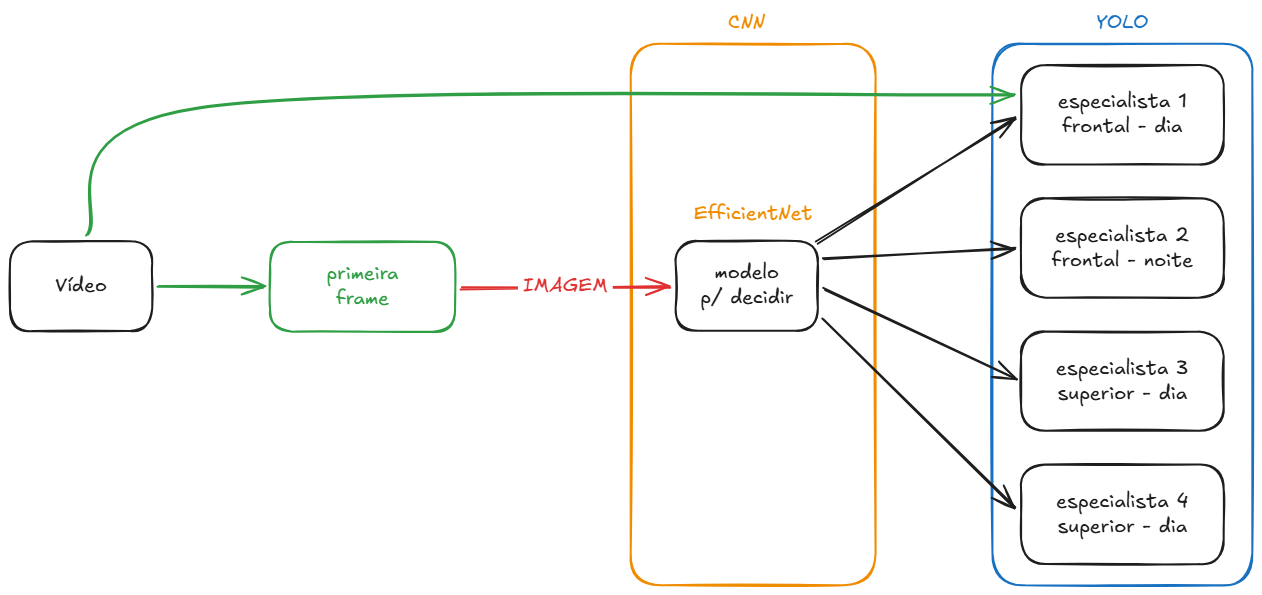
\includegraphics[height=7.2cm]{figures/moe.png}%
\caption{Arquitetura MoE proposta.}
\label{fig:moe_architecture}
{\footnotesize\centering Fonte: Autor (2026)\par}
\label{fig1}%
\end{center}
\end{figure}


\section{RESULTADOS}

Nesta seção, são apresentados e analisados os resultados experimentais obtidos durante o desenvolvimento do sistema.

\subsection{Análise Descritiva do Dataset Inicial e Falha da PoC}
\label{subsec:analise_poc}

Os testes preliminares basearam-se na inferência direta do modelo genérico YOLOv8 pré-treinado no conjunto de dados COCO \cite{journals/corr/LinMBHPRDZ14}. Uma vez que o referido \textit{dataset} não possui uma classe específica para caprinos, utilizou-se a classe morfologicamente semelhante \texttt{sheep} (ovelha). Conforme observado na Figura ~\ref{fig:poc_yolo}, os resultados mostraram-se insatisfatórios: o modelo foi incapaz de detectar a totalidade do rebanho confinado na baia principal, identificando apenas dois indivíduos com limiares de confiança baixos ($0,27$ e $0,48$).

\begin{figure}[!htbp] %h or !htbp
\vspace{-2pt}
\begin{center}
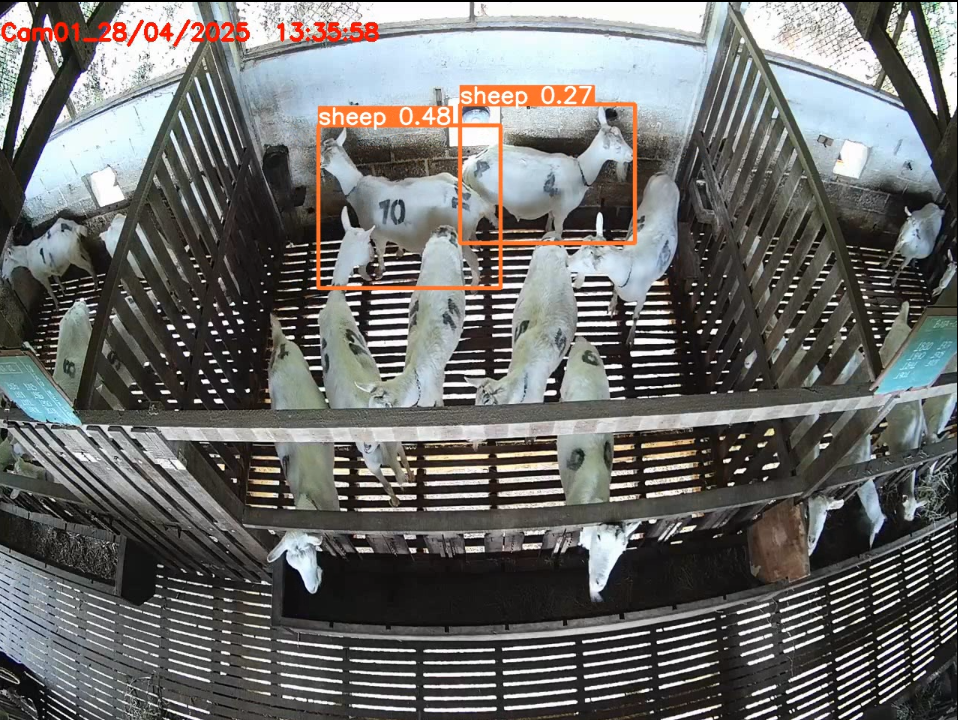
\includegraphics[height=6.2cm]{figures/sheep-test.png}%
\caption{Teste de classificação utilizando YOLOv8 sem treinamento com a classe \textit{sheep}.}
\label{fig:poc_yolo}
{\footnotesize\centering Fonte: Autor (2026)\par}
\label{fig2}%
\end{center}
\end{figure}

Este comportamento decorre da discrepância fenotípica entre as espécies e do viés geométrico induzido pelas perspetivas de capturas verticais. Testes adicionais variando cenários diurnos e noturnos confirmaram que modelos generalistas falham sob restrições severas de iluminação em ambiente confinado, fundamentando a necessidade da construção de uma base de dados própria e especializada.

\subsection{Desempenho da Rede de Roteamento (Gating Network)}
\label{subsec:resultados_gating}

A rede de roteamento, baseada na arquitetura \textit{EfficientNet}, foi submetida ao treinamento para classificar as imagens de entrada entre os quatro cenários que definem os especialistas: \texttt{class\_1} (Frontal Dia), \texttt{class\_2} (Frontal Noite), \texttt{class\_3} (Superior Dia) e \texttt{class\_4} (Superior Noite). O processo de otimização foi projetado para até 50 épocas, contando com um mecanismo de interrupção precoce (\textit{Early Stopping}) para mitigar o sobreajuste.

O treinamento apresentou uma convergência veloz. O critério de parada foi ativado na época 9, a evolução detalhada do histórico de perdas (\textit{loss}) e da acurácia ao longo das iterações pode ser observada na Figura~\ref{fig:learning_curves}. O comportamento síncrono e descendente entre as curvas de treino e validação comprova a estabilidade do modelo e elimina o risco de \textit{overfitting}. Ao final da validação, as métricas de Precisão, Revocação e \textit{F1-Score} atingiram o valor de $1.00$ para um conjunto total de 272 amostras de teste.

\vspace{-0.2cm}

\begin{figure}[!ht]
    \centering
    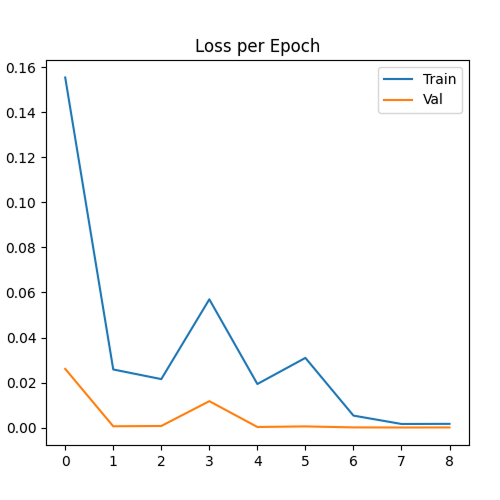
\includegraphics[width=0.45\textwidth]{figures/learning_curves.png}
    \caption{Curvas de aprendizado da Rede de Roteamento: (esquerda) Perda por época e (direita) Acurácia por época.}
    \label{fig:learning_curves}
    {\footnotesize Fonte: Autor (2026)\par}
\end{figure}

Após o treinamento foi utilizado o Occlusion a fim de compreender os pontos vitais para a classificação da imagem. Como pode-se observar na Figura ~\ref{fig:occlusion_blended}, os pontos mais claros demonstram as regiões mais relevantes para a classificação. Com isso, nota-se que pontos do ambiente como o padrão identificado nas paredes e o cercado que envolvem a baia foram pontos determinantes para identificar o tipo de imagem.

\begin{figure}[!ht]
    \centering
    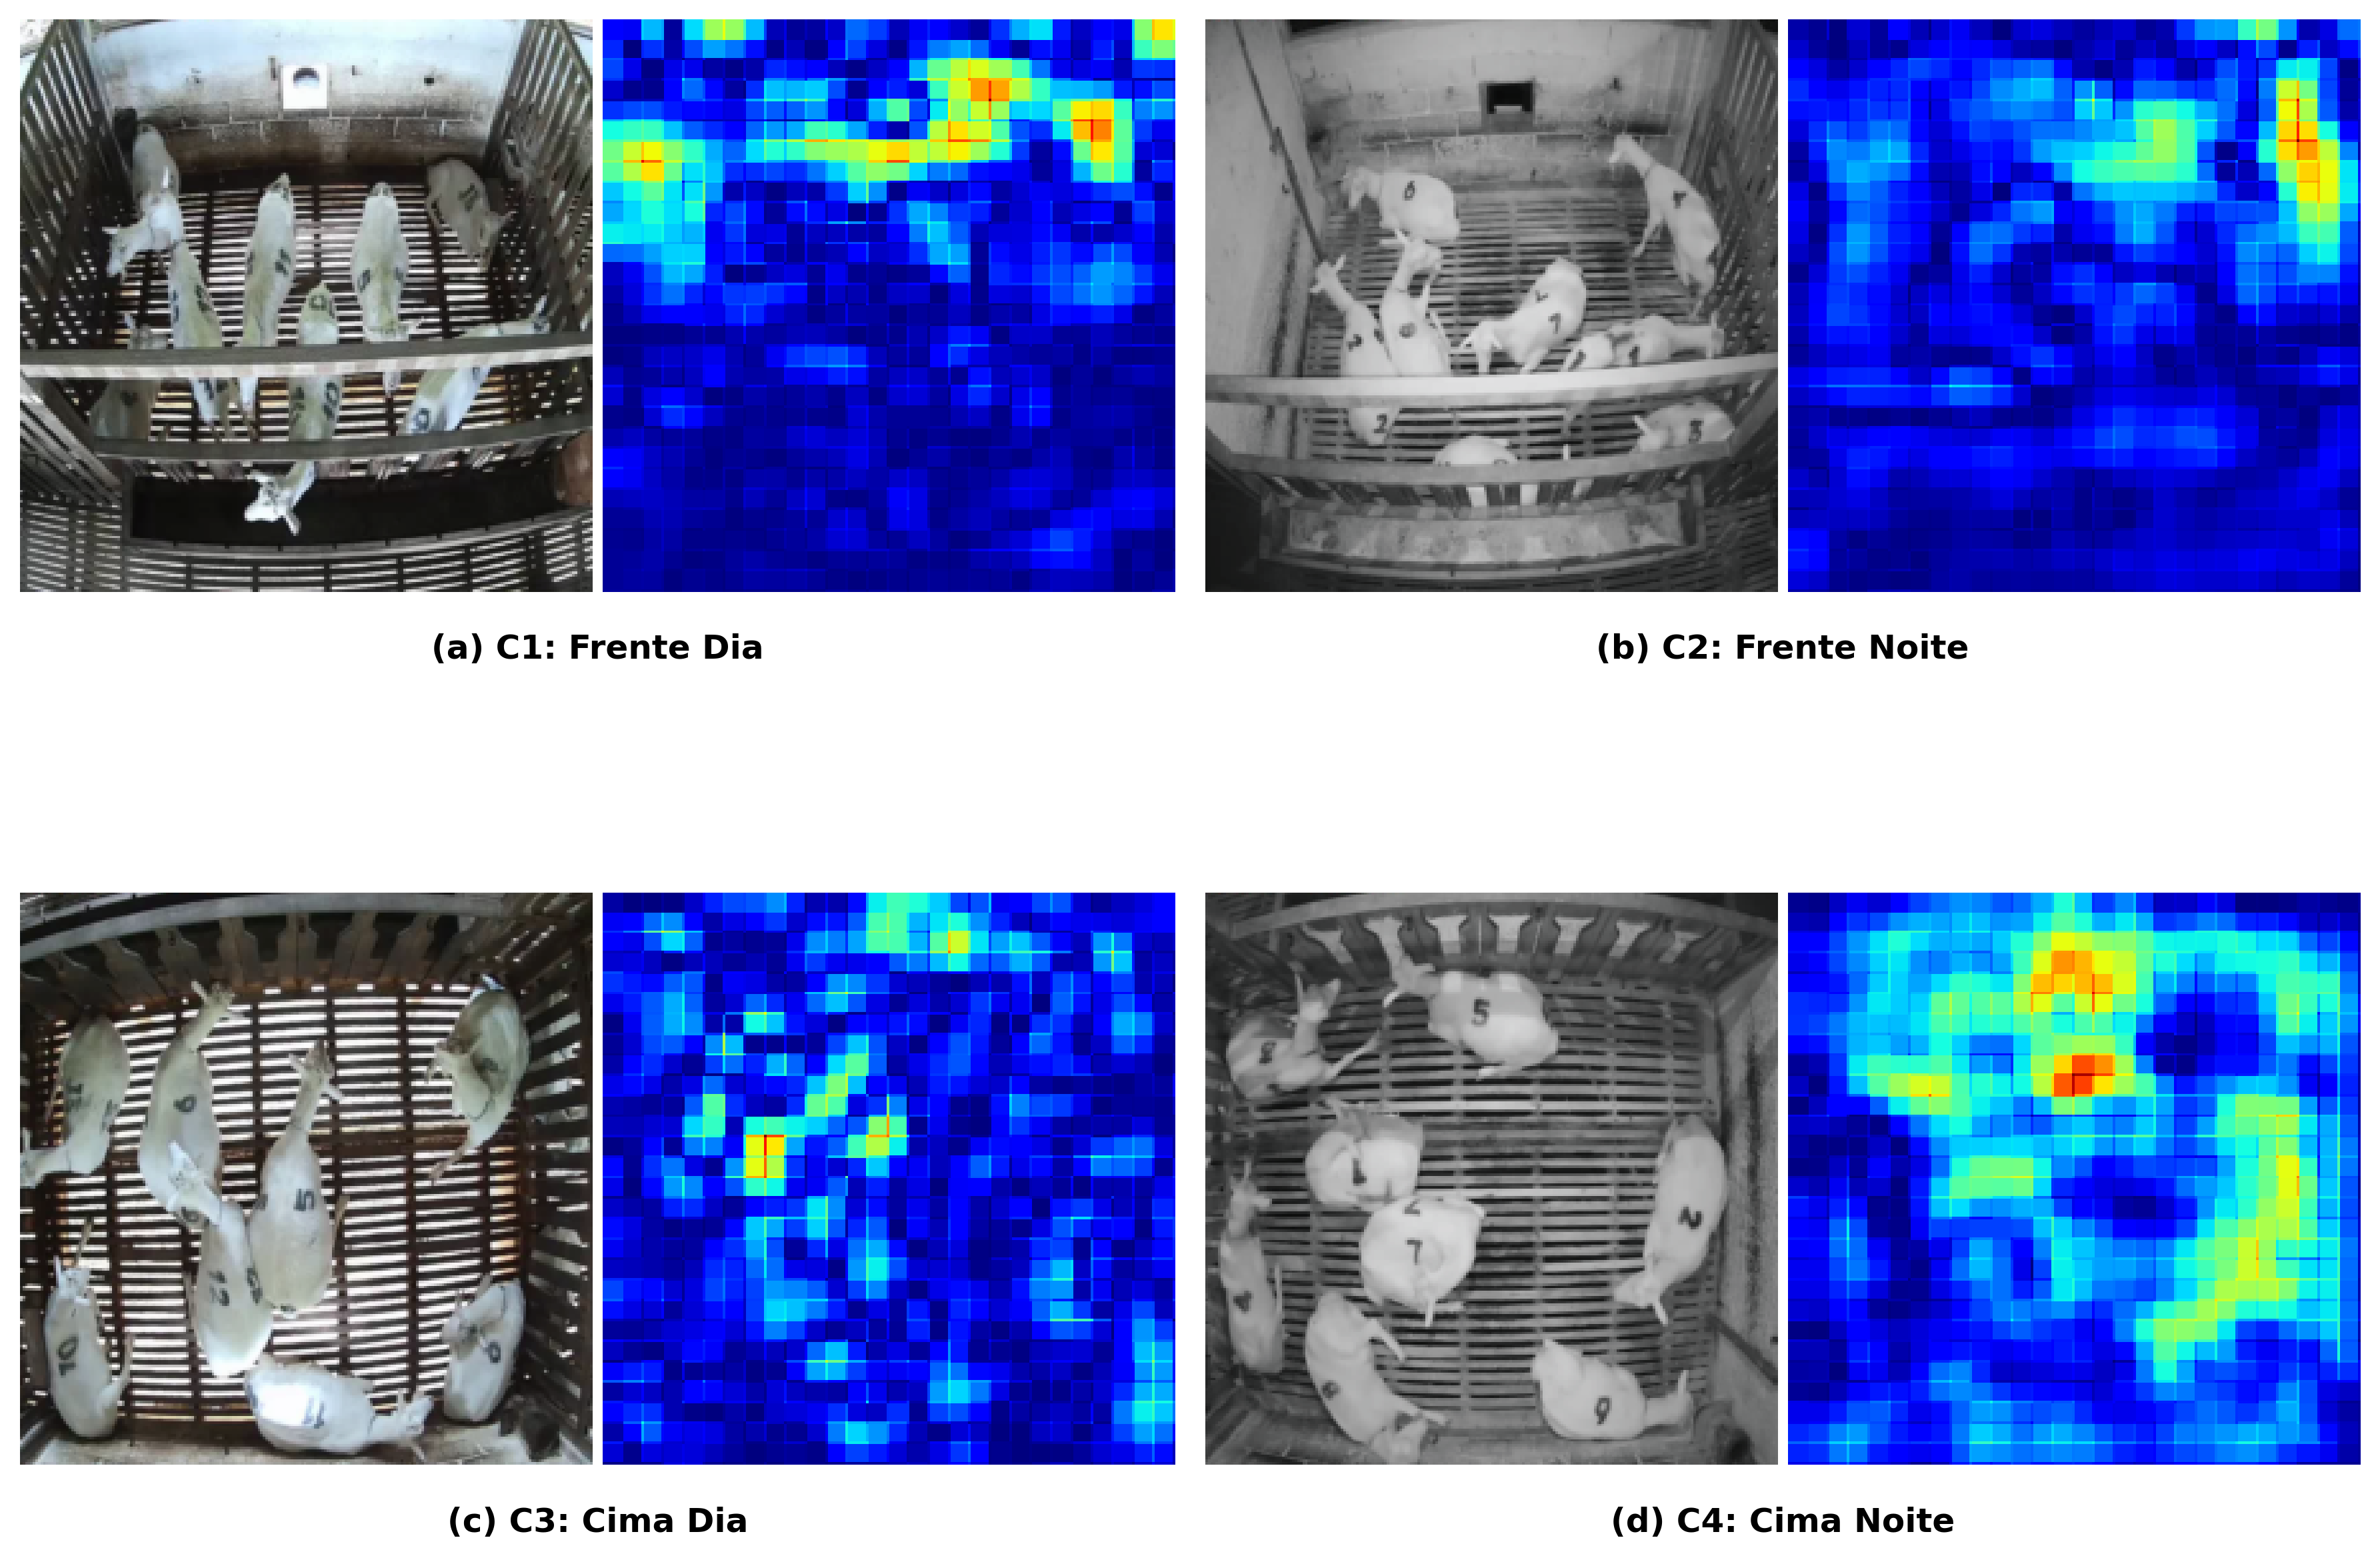
\includegraphics[width=0.91\textwidth]{figures/occlusion_blended.png}
    \caption{Aplicação do Occlusion para avaliar o comportamento da Rede de Roteamento.}
    \label{fig:occlusion_blended}
    {\footnotesize Fonte: Autor (2026)\par}
\end{figure}

Esse resultado se justifica pela simplicidade de realizar a classificação, mesmo diante de variações de iluminação e de potenciais desafios de oclusão parcial dos animais, a extração de características globais feita pela \textit{EfficientNet} provou ser resistente a essas interferências. Esse comportamento robusto assegura que o direcionamento dos \textit{frames} para os modelos especialistas YOLOv8 seja condizente.

\subsection{Análise do Treinamento dos Modelos Especialistas utilizando o K-Fold}
\label{subsec:treinamento_especialistas}

Conforme mencionando previamente, cada modelo especialista foi submetido a um processo de validação cruzada com $k=5$ partições. Essa estratégia garante que o pipeline de detecção seja exposto a diferentes subconjuntos de dados, mitigando o risco de \textit{overfitting} e validando a capacidade de generalização da rede em cenários específicos de iluminação (dia e noite) e perspectiva (frontal e superior).

A Tabela~\ref{tab:yolo_especialistas} consolida as métricas de desempenho alcançadas pelos melhores \textit{folds} de cada modelo especialista YOLOv8. São reportados os índices de Precisão (P), Revocação (R), \textit{F1-Score}, além das métricas padrão de avaliação de detectores de objetos: a precisão média de corte (\textit{mean Average Precision}) em $IoU = 0.50$ ($mAP_{50}$) e expandida no intervalo de $0.50$ a $0.95$ ($mAP_{50-95}$).

\begin{table}[H]
\caption{Métricas dos Melhores Folds dos Modelos YOLOv8 Especialistas.}
\label{tab:yolo_especialistas}
\centering{}
\begin{tabular*}{\textwidth}{@{\extracolsep{\fill}}llcccccc}
\hline
Especialista & Precisão (P) & Revocação (R) & F1-Score & mAP50 & mAP50-95 \\
\hline
Frontal Dia & 0.9966 & 0.9975 & 0.9971 & 0.9950 & 0.9015 \\
Frontal Noite & 0.9972 & 0.9968 & 0.9970 & 0.9950 & 0.8821 \\
Superior Dia & 0.9999 & 0.9995 & 0.9997 & 0.9950 & 0.8645 \\
Superior Noite & 0.9978 & 0.9972 & 0.9975 & 0.9950 & 0.8338 \\
\hline
\end{tabular*}
{\footnotesize\centering Fonte: Autor (2026)\par}
\end{table}

Os resultados experimentais demonstram alta consistência e acurácia em todos os cenários analisados, com $mAP_{50}$ saturado em $0,9950$ nos quatro especialistas. Observa-se, no entanto, variação relevante na dinâmica de convergência: o especialista Superior Noite atingiu seu pico de desempenho já na época 13, seguido por Superior Dia (época 50), Frontal Noite (época 81) e, por último, Frontal Dia (época 108). Os cenários noturnos, capturados sob espectro infravermelho, tendem a apresentar menor variabilidade visual de fundo e maior homogeneidade de textura, o que favorece a rápida convergência do especialista Superior Noite; essa vantagem, contudo, não se generaliza de forma determinística entre todos os cenários noturnos, uma vez que o especialista Frontal Noite convergiu mais lentamente que o Superior Dia -- evidenciando que a perspectiva de captura (frontal vs. superior) também desempenha papel relevante na dificuldade de ajuste, possivelmente em função da maior proximidade e sobreposição entre indivíduos característica da visão frontal frente à vista aérea.

Em termos da métrica mais rigorosa ($mAP_{50-95}$), o especialista Frontal Dia obteve o maior valor entre os quatro ($0,9015$), seguido por Frontal Noite ($0,8821$), Superior Dia ($0,8645$) e Superior Noite ($0,8338$). A contração observada nos cenários de perspectiva superior/zenital em relação aos frontais é consistente com o desafio geométrico de caixas delimitadoras menores e mais sobrepostas nessa perspectiva, na qual os animais tendem a se agrupar em torno do cocho de alimentação. Em síntese, os elevados valores de $mAP_{50}$ obtidos por todos os especialistas demonstram a eficácia da clusterização modular dos cenários, fornecendo uma base preditiva robusta para a rede de roteamento (\textit{Gating Network}) da arquitetura MoE global, apresentada na Figura~\ref{fig:moe_architecture}.

\subsection{Comparação com o Baseline Monolítico Generalista}
\label{subsec:baseline_overall}

Para estabelecer um ponto de comparação metodologicamente rigoroso para a arquitetura MoE -- em substituição ao teste preliminar de inferência direta sem treinamento discutido na Seção~\ref{subsec:analise_poc}, que teve caráter apenas motivacional e não constitui um baseline válido -- foi treinado um modelo monolítico generalista: um único YOLOv8m ajustado sobre a união das imagens dos quatro cenários (8.604 imagens, Tabela~\ref{tab:dataset_caracterizacao}), sem qualquer roteamento ou especialização por contexto de captura. O treinamento seguiu exatamente o mesmo protocolo de validação cruzada temporal descrito na Seção~\ref{subsec:temporal_kfold} ($K=5$, zona de purga de 15 quadros) e os mesmos hiperparâmetros da Seção~\ref{subsec:config_modelo} ($imgsz=640$, \textit{batch size} automático, \textit{patience}=30), garantindo que a comparação isole o efeito da arquitetura (monolítica vs. MoE) e não o efeito de protocolos experimentais distintos. Este baseline representa a alternativa direta mais simples à arquitetura MoE: um único detector aprendendo simultaneamente todas as combinações de perspectiva e iluminação, sem qualquer mecanismo de roteamento.

A Tabela~\ref{tab:baseline_overall} apresenta os resultados do baseline monolítico ao longo dos 5 \textit{folds} temporais.

\begin{table}[H]
\caption{Métricas do Baseline Monolítico (YOLOv8m Único, Dataset Unificado) por Fold.}
\label{tab:baseline_overall}
\centering{}
\begin{tabular*}{\textwidth}{@{\extracolsep{\fill}}lcccccc}
\hline
Fold & Precisão (P) & Revocação (R) & F1-Score & mAP50 & mAP50-95 \\
\hline
Fold 1 & 0.9914 & 0.9938 & 0.9926 & 0.9944 & 0.8700 \\
Fold 2 & 0.9945 & 0.9942 & 0.9943 & 0.9948 & 0.8707 \\
Fold 3 & 0.9977 & 0.9986 & 0.9982 & 0.9950 & 0.8965 \\
Fold 4 & 0.9967 & 0.9971 & 0.9969 & 0.9950 & 0.8839 \\
Fold 5 & 0.9939 & 0.9948 & 0.9943 & 0.9949 & 0.8653 \\
\hline
\textbf{Média} & \textbf{0.9948} & \textbf{0.9957} & \textbf{0.9953} & \textbf{0.9948} & \textbf{0.8773} \\
\hline
\end{tabular*}
{\footnotesize\centering Fonte: Autor (2026)\par}
\end{table}

Comparando os resultados do baseline monolítico com aqueles obtidos pelos modelos especialistas, observa-se que ambas as abordagens atingem valores elevados de mAP50, próximos do teto da métrica. Na métrica mais rigorosa, mAP50--95, também são observadas diferenças relativamente pequenas entre as abordagens. Esses resultados indicam que, no atual estágio de maturidade do dataset, um único YOLOv8m é capaz de aprender uma
representação conjunta competitiva das diferentes combinações de perspectiva e iluminação. Dessa forma, os resultados não demonstram superioridade generalizada da arquitetura MoE em termos das métricas agregadas de detecção.

A contribuição da arquitetura MoE, portanto, não reside primariamente em um ganho bruto de mAP sobre o baseline monolítico nesse regime de dados, mas em vantagens estruturais que a comparação de métricas agregadas não captura isoladamente: (i) \textbf{modularidade e escalabilidade} -- novos cenários de captura podem ser incorporados adicionando um novo especialista e uma nova classe à rede de roteamento, sem a necessidade de retreinar o modelo generalista completo; (ii) \textbf{isolamento de falhas} -- dificuldades específicas de um cenário, como a maior contração de mAP50-95 observada nos especialistas de perspectiva superior (Seção~\ref{subsec:treinamento_especialistas}), ficam confinadas ao especialista correspondente, sem risco de contaminar os pesos aprendidos para os demais cenários; e (iii) \textbf{explicabilidade do processo de decisão} -- a rede de roteamento fornece um sinal interpretável (o cenário identificado) sobre qual especialização foi ativada para cada inferência, validado pela análise de sensibilidade por oclusão da Seção~\ref{subsec:resultados_gating}, sem equivalente direto em um detector monolítico único.

Para além das métricas agregadas de validação cruzada, a diferença estrutural entre as duas abordagens torna-se evidente ao inspecionar a contagem de caixas delimitadoras produzidas em inferência sobre os mesmos quatro vídeos de teste independentes ilustrados na Figura~\ref{fig:comparacao_overall_moe}, cuja ausência de sobreposição com as sessões de treinamento foi previamente confirmada por comparação de similaridade entre quadros. Cada vídeo possui 80 quadros e registra o rebanho fixo de 8 indivíduos (Seção~\ref{subsec:aquisicao_dados}), de modo que o número de caixas esperado, na ausência de erros de detecção, é de $8 \times 80 = 640$ por vídeo. A inferência foi executada para as duas abordagens sob os mesmos limiares de confiança e de IoU de supressão não-máxima (NMS) ($conf=0{,}7$; $iou=0{,}7$).

A Tabela~\ref{tab:contagem_caixas} apresenta o total de caixas detectadas por vídeo em cada abordagem.

\begin{table}[H]
\caption{Total de Caixas Detectadas nos Vídeos de Teste: Baseline Overall vs. MoE.}
\label{tab:contagem_caixas}
\centering{}
\begin{tabular*}{\textwidth}{@{\extracolsep{\fill}}lcccc}
\hline
Cenário & Overall & MoE & Esperado ($8 \times 80$) \\
\hline
Frente Dia & 623 & 640 & 640 \\
Frente Noite & 643 & 640 & 640 \\
Cima Dia & 532 & 640 & 640 \\
Cima Noite & 663 & 640 & 640 \\
\hline
\end{tabular*}
{\footnotesize\centering Fonte: Autor (2026)\par}
\end{table}

O especialista MoE correspondente a cada cenário produziu exatamente as 640 caixas esperadas em todos os 4 vídeos ($100\%$ de acerto na contagem, com variância nula entre quadros), enquanto o baseline monolítico oscilou tanto para cima quanto para baixo do valor esperado, a depender do cenário. Uma inspeção quadro a quadro revela dois padrões de erro distintos no baseline: em \textit{Cima Dia}, a contagem nunca atinge 8 caixas em nenhum dos 80 quadros (variando entre 5 e 7), sugerindo subdetecção sistemática por oclusão entre indivíduos agrupados na vista zenital; já em \textit{Cima Noite} e, em menor grau, em \textit{Frente Noite}, ocorre o padrão oposto -- 26 dos 80 quadros de \textit{Cima Noite} (e 4 dos 80 de \textit{Frente Noite}) apresentam mais de 8 caixas (até 10), com sobredetecção causada por múltiplas caixas de alta confiança sobrepostas ao mesmo indivíduo. A verificação da sobreposição geométrica (\textit{Intersection over Union}) entre pares de caixas nesses quadros confirma a hipótese: caixas duplicadas sobre o mesmo animal chegam a $IoU = 0{,}64$, valor abaixo do limiar de supressão não-máxima utilizado ($iou=0{,}7$) e, portanto, não eliminado pelo pós-processamento padrão.

A Figura~\ref{fig:comparacao_overall_moe} ilustra esse comportamento nos quatro cenários operacionais, sempre comparando o baseline monolítico (coluna esquerda) com o especialista MoE correspondente (coluna direita) no mesmo quadro do mesmo vídeo de teste. Em \textit{Frente Dia} (painéis a-b) e \textit{Cima Dia} (painéis e-f), o baseline deixa de detectar parte do rebanho (6 e 5 caixas, respectivamente, ante as 8 esperadas), enquanto o especialista MoE localiza os 8 indivíduos em ambos os casos. Em \textit{Frente Noite} (painéis c-d) e \textit{Cima Noite} (painéis g-h), o padrão se inverte: o baseline atribui duas caixas de alta confiança ($\geq 0{,}73$) a um mesmo indivíduo, ao passo que o especialista MoE correspondente delimita cada um dos 8 indivíduos com exatamente uma caixa, sem duplicações. Em conjunto, os quatro pares de painéis evidenciam que a instabilidade na contagem do baseline monolítico -- seja por subdetecção, seja por sobredetecção -- não é exclusiva de um único cenário, mas se manifesta de forma diferente em cada combinação de perspectiva e iluminação, ao passo que o especialista MoE mantém a contagem correta de forma consistente nos quatro casos.

\begin{figure}[!htbp]
\vspace{-2pt}
\begin{center}
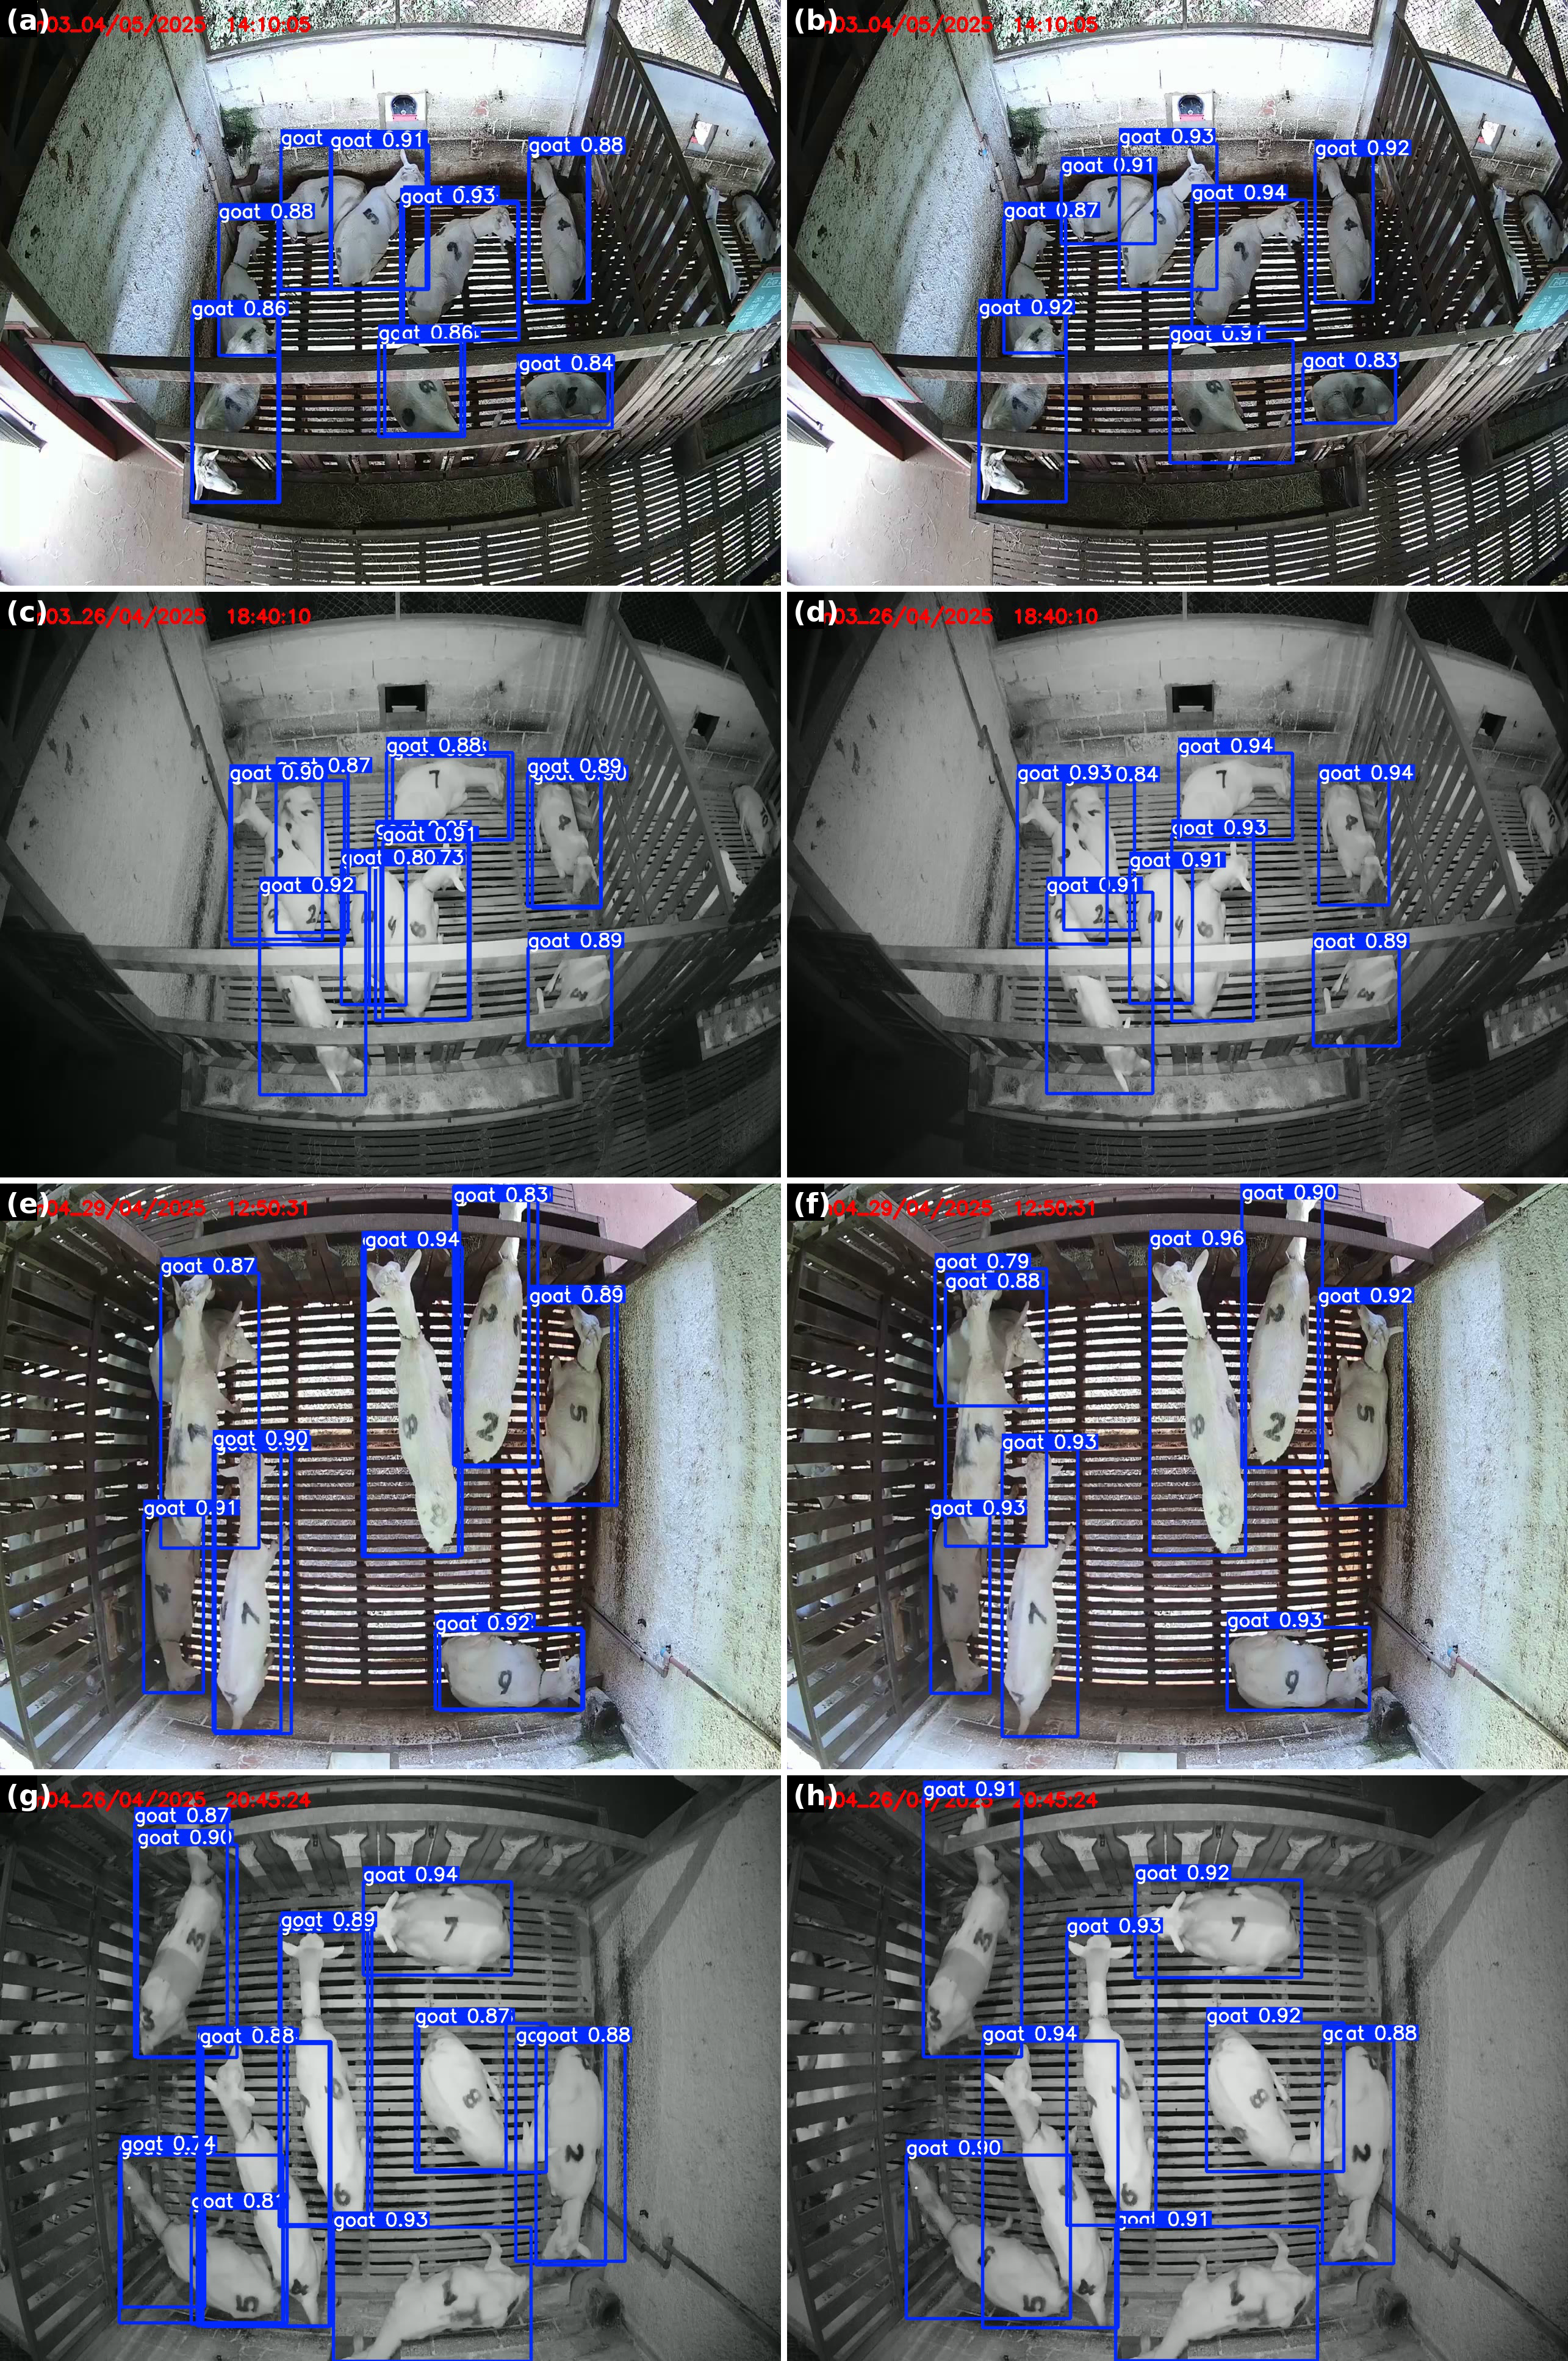
\includegraphics[width=0.85\textwidth]{figures/comparacao_overall_moe.png}%
\caption{Comparação lado a lado entre o baseline monolítico (esquerda) e o especialista MoE correspondente (direita), no mesmo quadro do mesmo vídeo de teste, nos quatro cenários operacionais: (a)-(b) \textit{Frente Dia}, quadro 10 (6 vs. 8 caixas); (c)-(d) \textit{Frente Noite}, quadro 55 (9 vs. 8 caixas); (e)-(f) \textit{Cima Dia}, quadro 62 (5 vs. 8 caixas); (g)-(h) \textit{Cima Noite}, quadro 6 (10 vs. 8 caixas). O valor esperado é de 8 caixas por quadro (Seção~\ref{subsec:aquisicao_dados}).}
\label{fig:comparacao_overall_moe}
{\footnotesize\centering Fonte: Autor (2026)\par}
\end{center}
\end{figure}

Vale notar que esse comportamento não é diretamente capturado pelas métricas agregadas de mAP reportadas nas Tabelas~\ref{tab:yolo_especialistas} e~\ref{tab:baseline_overall}: caixas duplicadas de alta confiança sobre um mesmo objeto tendem a ser parcialmente absorvidas pelo cálculo de precisão-revocação em múltiplos limiares de confiança que compõe o mAP, sem necessariamente penalizar a métrica agregada na mesma proporção em que penalizam a contagem bruta de detecções em um único limiar de operação fixo, como o utilizado nesta inspeção qualitativa. Esse resultado reforça, com evidência direta sobre vídeos de teste, a vantagem de isolamento de falhas discutida anteriormente: ao restringir cada especialista a um único domínio visual homogêneo, a arquitetura MoE elimina a ambiguidade de delimitação que emerge quando um único detector precisa generalizar simultaneamente sobre indivíduos visualmente semelhantes em diferentes condições de captura.

Em ambas as abordagens, apenas um modelo YOLOv8m é executado por quadro. No baseline generalista, o mesmo detector é utilizado em todos os cenários, enquanto na arquitetura MoE é executado apenas o especialista selecionado pela rede de roteamento. A rede de roteamento é utilizada uma única vez por vídeo ou sessão para determinar o especialista correspondente.

\subsection{Integração e Avaliação do Modelo Final}

A integração final da arquitetura de MoE unificou de forma síncrona a rede de roteamento baseada em \textit{EfficientNet} e os quatro modelos especialistas YOLOv8 customizados para as condições específicas de iluminação (Dia e Noite) e posicionamento de câmera (Frontal e Superior). Essa abordagem permite que o fluxo de processamento de vídeo seja otimizado dinamicamente em tempo de execução, direcionando as demandas computacionais apenas à sub-rede mais qualificada para o contexto observado.

Os resultados obtidos ao longo das etapas anteriores evidenciam que a adoção da arquitetura baseada em MoE vai além de uma simples divisão do problema em submodelos independentes. A estratégia proposta explora a especialização de cada detector para um contexto específico de captura, reduzindo a variabilidade que cada modelo precisa aprender e permitindo que os parâmetros sejam ajustados para distribuições de dados mais homogêneas. Dessa forma, a rede de roteamento atua apenas como um mecanismo de seleção do especialista mais adequado ao cenário identificado, enquanto a etapa de detecção permanece restrita ao modelo treinado para aquela condição de perspectiva e iluminação. Essa organização modular também amplia a escalabilidade da solução, pois novos especialistas podem ser incorporados futuramente para contemplar outros cenários de aquisição, sem a necessidade de retreinar toda a arquitetura.

Com essa configuração, o resultado prático das inferências geradas pelo modelo completo nos quatro cenários que compõem o ecossistema do confinamento -- visão frontal diurna, visão frontal noturna operando sob espectro infravermelho, visão superior diurna sob a incidência de luz natural e visão superior noturna -- pode ser observado diretamente nos painéis do especialista MoE já apresentados na Figura~\ref{fig:comparacao_overall_moe} (painéis b, d, f e h, correspondentes a cada um desses quatro cenários, respectivamente).

Como pode ser observado pelas caixas envolventes (\textit{bounding boxes}) geradas nesses painéis, o acoplamento sistêmico mitigou com sucesso as falhas críticas diagnosticadas na Prova de Conceito (Seção~\ref{subsec:analise_poc}). Mesmo diante de oclusões parciais severas causadas pela proximidade dos animais no cocho de alimentação (cenários diurnos, painéis b e f) ou da sobreposição geométrica inerente à perspectiva vertical superior (painéis f e h), os especialistas registraram altos índices de confiança preditiva: considerando a totalidade das $2.560$ caixas detectadas nos quatro vídeos de teste ($640$ por vídeo, Tabela~\ref{tab:contagem_caixas}), a confiança variou entre $0,74$ e $0,96$, com média de $0,91$.

%%Em termos de desempenho sistêmico, o acoplamento não gerou prejuízo computacional, uma vez que a rede de roteamento atua como um classificador global extremamente leve de passo único, ativando estritamente um único especialista YOLOv8 de acordo com a primeira \textit{frame}.

\section{CONCLUSÃO}

O presente trabalho apresentou o desenvolvimento e a avaliação de uma arquitetura baseada em Mistura de Especialistas (\textit{Mixture of Experts} -- MoE) voltada à detecção automatizada de caprinos da raça \textit{Saanen} em ambientes de confinamento. A estratégia combina uma rede de roteamento baseada em \textit{EfficientNet}, responsável pela classificação do cenário de captura, com quatro modelos YOLOv8 especializados em diferentes combinações de perspectiva e iluminação. Os resultados obtidos demonstraram elevado desempenho dos especialistas nos quatro cenários avaliados, indicando a viabilidade da abordagem modular para a detecção de caprinos sob diferentes condições de captura.

A comparação com o modelo YOLOv8m monolítico treinado sobre a união dos quatro cenários mostrou que ambas as abordagens apresentaram desempenho elevado e semelhante nas métricas agregadas de detecção. Dessa forma, os resultados obtidos até o presente estágio do projeto não demonstram superioridade generalizada da arquitetura MoE em termos de mAP. Sua principal contribuição está associada à especialização dos detectores por condição de captura e à organização modular da solução, permitindo tratar separadamente diferentes combinações de perspectiva e iluminação.

%%O presente trabalho apresentou o desenvolvimento e a validação de uma arquitetura baseada em Mistura de Especialistas (\textit{Mixture of Experts} - MoE) voltada à detecção e localização automatizada de caprinos da raça \textit{Saanen} em ambientes de confinamento. A estratégia adotada mostrou-se eficaz e superior às abordagens tradicionais de modelos genéricos unificados. 

A principal contribuição deste estudo reside na proposição de um ecossistema computacional modular aplicado à Zootecnia de Precisão, voltado à detecção de caprinos em diferentes condições de captura. A abordagem permite organizar modelos especialistas de acordo com características específicas do ambiente, reduzindo a necessidade de um único detector lidar simultaneamente com diferentes perspectivas e condições de iluminação.

%%A principal contribuição deste estudo reside na formulação de um ecossistema computacional modular e de baixo custo aplicado à Zootecnia de Precisão, preenchendo uma lacuna crítica na literatura decorrente da escassez de bases de dados específicas para caprinos. Cientificamente, o trabalho demonstra que a rede de roteamento (\textit{gating network}) baseada em \textit{EfficientNet} aprendeu características estruturais globais do ambiente confinado, alcançando boa acurácia e robustez a ruídos visuais, conforme validado pelos testes de Occlusion. Esse direcionamento permitiu que os quatro especialistas YOLOv8 customizados apresentassem elevada confiança preditiva ($0,84$ a $0,95$) e estabilidade estatística comprovada por validação cruzada ($K$-\textit{Fold}).

%%Do ponto de vista prático e de engenharia computacional, o acoplamento síncrono das sub-redes não gerou gargalos de processamento. Uma vez que a CNN atua como um filtro leve de passo único e apenas um especialista é ativado de acordo com a primeira \textit{frame}, o consumo de memória e o esforço computacional foram mitigados.

Como trabalhos futuros, propõe-se expandir o ecossistema do modelo para incluir o rastreamento individualizado dos animais ao longo do tempo (\textit{multi-object tracking}), viabilizando a análise comportamental de bem-estar animal. Além disso, a arquitetura atual é escalável, de forma que caso seja necessário incluir um novo cenário e adicionar um novo especialista, ele pode ser adicionado realizando o seu treinamento de forma separada e o incluindo na CNN, garantindo a modularidade e assegurando que os outros especialistas não serão afetados nessa atualização.

\subsection*{\textit{Agradecimentos}}

Os autores agradecem à Universidade Federal de Juiz de Fora (UFJF), à Universidade Federal de São João del-Rei (UFSJ) e ao Departamento de Zootecnia da UFSJ pelo suporte no desenvolvimento deste trabalho.

Os autores utilizaram a ferramenta ChatGPT (OpenAI) para auxiliar na revisão linguística e na depuração do código computacional utilizado nos experimentos do manuscrito. Todo o conteúdo científico, a interpretação dos resultados e as conclusões permanecem sob responsabilidade dos autores.

\bibliographystyle{apalike}
\fontsize{11}{0}\selectfont
\bibliography{bib/references}
\vspace{0.5cm}

\begin{center}
\textbf{ARTIFICIAL INTELLIGENCE APPLIED TO GOAT DETECTION IN CONFINED ENVIRONMENTS}   
\end{center}

\vspace{0.1cm}

\begin{abstract}
The use of Computer Vision-based systems has expanded considerably in recent years, with promising applications in precision livestock farming, including the automated monitoring and analysis of animals in confined environments. Despite the widespread availability of technological resources, challenges remain in applying these systems under real-world conditions, particularly in the presence of variations in viewpoint and illumination. In this context, this study proposes a Mixture of Experts (MoE) architecture for the detection of Saanen goats in confined environments. The proposed approach combines a routing network (gating network) based on EfficientNet -- responsible exclusively for classifying the capture scenario (viewpoint and illumination condition), and not for classifying the animal itself -- with four YOLOv8 models, each dedicated to detecting the single target class \texttt{goat} under a specific combination of viewpoint and illumination condition. For training and evaluation of the detectors, videos captured in experimental environments at the Federal University of São João del-Rei were used to construct a labeled image dataset containing a single target class, \texttt{goat}. The results indicated high performance of the specialized models across the four evaluated scenarios, demonstrating the feasibility of the proposed modular strategy for goat detection under different capture conditions.
\end{abstract}

\keywords{\em{Artificial Intelligence, Computer Vision, Object Detection, Mixture of Experts (MoE), Precision Livestock Farming.}}

\end{document}